% This is samplepaper.tex, a sample chapter demonstrating the
% LLNCS macro package for Springer Computer Science proceedings;
% Version 2.20 of 2017/10/04
%
\documentclass[runningheads]{llncs}
%
\usepackage{graphicx}
% Used for displaying a sample figure. If possible, figure files should
% be included in EPS format.
%
% If you use the hyperref package, please uncomment the following line
% to display URLs in blue roman font according to Springer's eBook style:
% \renewcommand\UrlFont{\color{blue}\rmfamily}

\begin{document}
%
\title{A review of a hybrid feature selection method for DNA microarray data}
%
%\titlerunning{Abbreviated paper title}
% If the paper title is too long for the running head, you can set
% an abbreviated paper title here
%
\author{Laura Rodríguez-Navas\orcidID{0000-0003-4929-1219}}
%
% \authorrunning{F. Author et al.}
% First names are abbreviated in the running head.
% If there are more than two authors, 'et al.' is used.
%
\institute{Universidad Internacional Menéndez Pelayo (UIMP), Madrid, Spain \\
	\email{rodrigueznavas@posgrado.uimp.es}}
%
\maketitle              % typeset the header of the contribution
%
\begin{abstract}
The emergence of DNA Microarray technology has enabled researchers to analyse the expression level of thousands of genes simultaneously. The Microarray data analysis is the process of finding the most informative genes as well as remove redundant and irrelevant genes. One of the most important applications of Microarray data analysis is cancer classification. Gene expression profiles, which represent the state of a cell at a molecular level, have great potential as a medical diagnosis tool. In cancer classification, available training data sets are generally of a small sample size compared to the number of genes involved. Along with training data limitations, this constitutes a challenge to certain classification methods. However, the curse of dimensionality and the curse of sparsity make classifying gene expression profiles a challenging task. One of the most effective methods to overcome these challenges is feature (gene) selection. The feature (gene) selection can be used to successfully extract those genes that directly influence classification accuracy and to eliminate genes that have no influence on it. This significantly improves calculation performance and classification accuracy. In this paper, I aim to review the correlation-based feature selection (CFS) and the Taguchi-genetic algorithm (TGA) that are merged into a new hybrid method, since the classification accuracy obtained by the reviewed hybrid method is higher, compared to other classification methods from the literature.

\keywords{Feature selection \and Taguchi-genetic algorithm \and Leave-one-out cross-validation.}

\end{abstract}
%
%
%
\section{Introduction}

DNA Microarray technology is a powerful tool that helps researchers to monitor the gene expression level in an organism. Microarray data analysis provides valuable results which contribute towards solving gene expression profile problems. One of the most important applications of Microarray data analysis is cancer classification. Cancer may be a genetic disease; the analysis of cancer pathology in the analysis of genes that cause cancer, i.e. the gene mutation that is responsible for cancer and reflects the changes in the expression level of various genes. However, classifying the gene expression profile is a challenging task and considered as (NP)-Hard problem~\cite{narendra1977branch}. Hence, not all genes contribute to the presence of cancer. A vast number of genes are irrelevant or insignificant to clinical cancer diagnosis. Therefore, incorrect diagnoses can be reached when all the genes are used in the Microarray gene expression classification. There are two main issues related to the analysis of the Microarray data; first, the dataset in the Microarray is high-dimensional which means it contains several thousand genes (features) and it has low data sparsity, meaning it has a low number of samples, usually tens of samples. Second, gene expression data has a high complexity; genes are directly or indirectly correlated to each other. Standard machine learning methods do not perform well, because these methods are best suited when there are more samples than features.

To overcome these issues, dimension reduction or feature (gene) selection algorithms have been applied. Generally, gene selection methods are categorized into three categories: filter, wrapper and embedded. The filter approach separates data before the actual classification process takes place and then calculates feature weight values, and thus features that accurately present the original data set can be identified. However, a filter approach does not account for interactions amongst the features. The method in the filter approach category is described in section~\ref{Correlation-based feature selection}. Wrapper models, on the other hand, generally are focused on improving classification accuracy of pattern classification problems and typically perform better (i.e., reach higher classification accuracy) than filter models. However, wrapper approaches are more computationally expensive than filter methods. Several methods in this category have previously been used to perform feature selection of training and testing data, such as genetic algorithm (GA) which is described in section~\ref{Genetic algorithm}. And the embedded techniques use an inductive algorithm. The inductive algorithm itself represents the feature selector and the classifier, searching for an optimal subset of features that are built into the classifier. The advantage of embedded algorithms is that they take the interaction with the classifier into account. A disadvantage of embedded algorithms is that they are generally based on a greedy mechanism, i.e., they only use top-ranked attributes to perform sample classification~\cite{saeys2007review,yang2010multi}.

Recently, hybrid and ensemble methods are added to the general framework of feature selection. A hybrid approach is built to take advantage of both filter and wrapper approaches. Thus, it combines the computational efficiency of the filter approach with the high performance of the wrapper approach. A hybrid feature selection approach consisting of two stages is presented in this paper. The first stage involves a filter approach that is used to calculate correlation-based feature weights for each feature, thus identifying relevant features. And the second stage constitutes a wrapper approach, i.e. the previously identified relevant feature subsets are tested by a Taguchi-genetic algorithm (TGA), which tries to determine optimal feature subsets. The optimal performance of the hybrid approach is dependent on two factors; the classification accuracy and the number of selected genes.

\section{Feature (gene) selection methods}

\subsection{Correlation-based feature selection}\label{Correlation-based feature selection}
Correlation-based feature selection (CFS) was developed by Hall in 1999~\cite{hall1998correlation}. CFS is a simple filter method that ranks features subsets, that is based on the correlation between the heuristic evaluation equation (\ref{heuristic evaluation equation}). CFS is used to select the best combination of attribute subsets via score values from the original data sets and the heuristic evaluation equation is employed to identify the best combination. 

The aim of CFS is to reduce the amount of feature to feature correlations while increasing the feature to class correlations. This paper use Weka~\cite{frank2004data} to implement the CFS and use the selected gene subsets to identify different cancer types and various diseases.

\begin{equation}\label{heuristic evaluation equation}
	Merit_{s} = \frac{k\bar{\gamma}_{cf}}{\sqrt{k+k(k-1)\bar{\gamma}_{ff}}}
\end{equation}
This is the heuristic evaluation equation where $Merit_{s}$ is the merit of feature subset $S$ containing $k$ features, $\bar{\gamma}_{cf}$ is the average feature and class correlation, and $\bar{\gamma}_{ff}$ is the average feature-feature intercorrelation ($f\in S$).

\subsection{Genetic algorithm}\label{Genetic algorithm}
A genetic algorithm (GA) was first developed by Holland in 1970. A GA is a stochastic search algorithm modelled on the process of natural selection underlying biological evolution. GA has been successfully applied to many searches, optimization, and machine learning~\cite{holland1975adaptation}. 

The main principle of the GA is to generate a population randomly while producing offspring with the same inherited characteristics. The algorithm has evolved into three operations: selection, crossover, and mutation. The selection operation chooses the fittest chromosomes, before allowing them to pass to the next generation. Within the crossover operation, two individuals are then selected via the selection operation process. For each individual crossover then, the operation will select a random crossover point and so the two individuals will swap to produce new offspring. And the mutations are necessary, for there to be a level of diversity maintained in the population. 

In this paper, it is proposed a Taguchi method described in section~\ref{Taguchi-Genetic Algorithm} and their optimization (described in section~\ref{CFS–TGA method}) that is based on the GA feature selection algorithm, just described.

\subsection{Taguchi-Genetic Algorithm}\label{Taguchi-Genetic Algorithm}
The Taguchi-Genetic Algorithm (TGA) is a hybridization of the Taguchi method and Genetic algorithm (GA) where the Taguchi method is inserted in the crossover and mutation operations. The TGA is normally used as a local search algorithm to select genes for crossover operations. 

The Taguchi method was developed by Genichi Taguchi and it is a statistical method of robust design where the processes or products can be analysed and improved by altering relevant design factors. The commonly used Taguchi method~\cite{tsai2004hybrid,taguchi1999robust,wu2000taguchi} provides two tools, an orthogonal array (OA) and a signal-to-noise ratio (SNR) for analysis and improvement. The OA used in this paper is a matrix arranged in rows and columns, with each column it is indicated a specific design parameter and each row represent an experimental trial with a combination of different levels for all design factors. This matrix provides a comprehensive analysis of interactions among a balanced set of experimentation runs and systematic comparisons of the different levels of each designed factors. In this paper, the SNR is used to determine the robustness of the levels of each design parameter and it is utilized to analyse and optimize the design parameters for the targets. Conceptually, SNR is represented as (\ref{SNR}) and a high SNR level by specifying design parameters represents good results for a particular target.

\begin{equation}\label{SNR}
	SNR = -10\log\left(\frac{1}{n}\sum_{t = 1}^{n}\frac{1}{y^2_{t}}\right)
\end{equation}

\section{CFS–TGA method}\label{CFS–TGA method}
Chuang et al.~\cite{chuang2011hybrid} proposed a new hybrid method for gene selection that combined Correlation-based Feature Selection (CFS) and the Taguchi-Genetic Algorithm (TGA). This method is the method proposed hybrid method in the paper and it is carried out in two stages. The first stage employs the correlation-based feature selection CFS filter method to remove irrelevant features. And the second stage involves a wrapper approach, employing the TGA methodology to the features that are generated from the filter stage and in doing so identify the best feature subset. Fig.~\ref{fig1} details the CFS–TGA method individual steps of the two stages.

\begin{figure}
	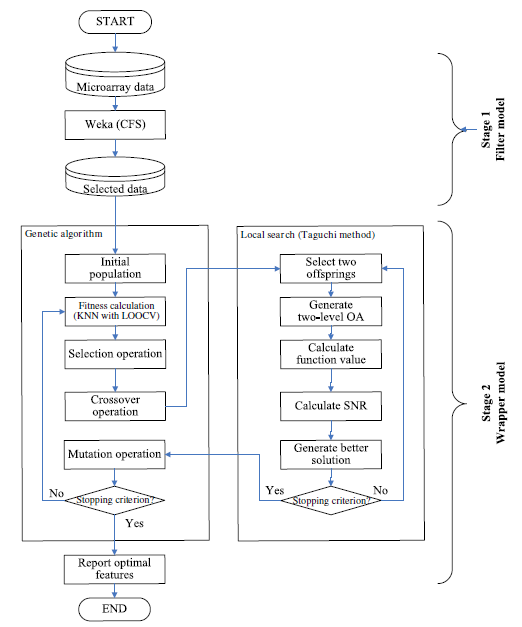
\includegraphics[width=\textwidth]{fig1}
	\caption{CFS–TGA method individual steps of two stages.}
	\label{fig1}
\end{figure}

The K-nearest neighbour (KNN) classifier~\cite{cover1967nearest,fix1985discriminatory} with Leave–One–Out Cross Validation (LOOCV) method~\cite{cawley2003efficient,stone1974cross} is used in the paper to evaluate the proposed hybrid method in terms of classification accuracy. Eleven cancer datasets with binary and multi-class are evaluated. Then, the result of the proposed hybrid method is compared with the result obtained by KNN, measured by the LOOCV method. The comparison shows that the proposed hybrid method achieves the highest classification accuracies in ten datasets where six datasets achieves an accuracy of 100\%.

Considering the result, it obvious that the hybrid method shows superior performance in terms of high accuracy and the small number of selected genes. This is because the hybrid algorithm deal perfectly with high dimensionality and overfitting problems by applying the filter approach first as a pre-processing step in order to reduce the dimensionality of the Microarray gene expression profiles.

\section{Conclusions}
How it is commented in the introduction, the Microarray cancer classification suffers from an overfitting problem. This is due to the curse of dimensionality: a small number of sample and many features. Thus, to avoid it I highly recommend applying the CFS–TGA method in order to adopt filtering before starting the classification process.

Moreover, in this type of problem, the parameters fitting is not an easy process. Because it affects classification accuracy. In cancer gene expression data classification, the parameter fitting is depending on the gene expression datasets and the applied feature selection and classification and methods. Thus, the different dataset has different parameters value, which is not fit for all algorithms. 

Microarray data analysis provides valuable results which contribute towards solving gene expression profile problems. As I mentioned before one of the most important applications of Microarray data analysis is cancer classification. Classification is challenging due to the high dimensionality found in a small sample size of gene expression data. The most practical method to overcome these challenges is therefore a feature selection technique that employs hybrid algorithms. In order to review and compare a hybrid algorithm with other types of algorithms from literature, I have chosen this paper. And I can conclude that among all other applied algorithms from the literature the CFS–TGA method achieves the highest accuracy with relatively small numbers of selected genes.

Therefore, as future work, I recommend applying this hybrid gene selection algorithm based on a filter and wrapper approach to identify the most informative genes for cancer classification.
%
% ---- Bibliography ----
%
% BibTeX users should specify bibliography style 'splncs04'.
% References will then be sorted and formatted in the correct style.
%
\bibliographystyle{splncs04}
\bibliography{samplepaper}
%
\end{document}
